\chapter{Pruebas}
\label{chap:pruebas}

En este capítulo se realizan pruebas con el fin de medir, cuantitativa y cualitativamente, las ventajas y/o desventajas que tiene el uso de Dagger para la gestión de un ciclo completo de CI/CD. Se proponen dos pruebas diferentes:

\begin{itemize}
  \item Ejecución de los tests \textit{end-to-end} con Dagger.
  \item Construcción y ejecución de tests de los paquetes de la aplicación. Tanto con Dagger como sin él.
\end{itemize}

En cada uno de los apartados dedicados a las diferentes pruebas se indica lo que implica realizarlos.

\section{Entorno de pruebas}

Las pruebas se realizan en un ordenador portátil con las siguientes características de \textit{software} y \textit{hardware}:

\begin{itemize}
  \item \textit{PC}: MacBook Air, 13-inch, 2024
  \item \textit{Chip}: Apple M3
  \item \textit{RAM}: 16 GB
  \item \textit{Sistema Operativo}: MacOs Sequoia 15.5
  \item \textit{Red}: Por cable, aproximadamente 1 GB simétrico.
\end{itemize}

Las versiones de los binarios utilizados se pueden encontrar en el Apéndice \ref{chap:usuario}.

\section{Prueba 1}

Lo que se pretende comprobar con esta prueba es ver cómo afecta el almacenamiento de caché que lleva a cabo Dagger tras varias ejecuciones de una función. Se realizarán medidas de tiempo bajo ciertas condiciones, con el fin de obtener diferentes valores y observar cuánto tiempo permite ahorrar Dagger gracias a su gestión de la caché. Se ejecuta varias veces la función \texttt{endtoend} implementada en el módulo de CI. Dicha función realiza las siguientes acciones:

\begin{itemize}
  \item Ejecuta los tests y el \textit{linting} del paquete del \textit{backend} de la aplicación.
  \item Realiza el \textit{linting} del \textit{frontend}.
  \item Levanta los servicios de ambos paquetes.
  \item Ejecuta los tests del \textit{frontend} con Cypress.
\end{itemize}

En definitiva, con la función que se va a utilizar en esta prueba, se realiza un testeo integral de toda la aplicación.

Antes realizar esta prueba se borra la caché que pudieran tener almacenada tanto de Dagger como de Docker. Para esto se utilizan los comandos del Listing \ref{lst:no-cache}.

\begin{listing}[!ht]
  \begin{minted}{bash}
dagger core engine local-cache prune

docker system prune -af
\end{minted}
\caption{Borrado de caché de Dagger y Docker.}
\label{lst:no-cache}
\end{listing}

Para probar la función, simplemente es necesario ejecutar el comando que se muestra en el Listing \ref{lst:endtoend}.

\begin{listing}[!ht]
  \begin{minted}{bash}
dagger call --sec-env=file://../../.env endtoend
\end{minted}
\caption{Testeo integral de la aplicación con el módulo de CI.}
\label{lst:endtoend}
\end{listing}

Se lanza el comando anterior cuatro veces, realizando un cambio en el código de la aplicación entre cada una de las ejecuciones. Esto tiene como finalidad evitar que se haga un uso total de la caché, debido a que Dagger comprueba los parámetros de entrada que se pasan a cada función (el código fuente, en este caso) para decidir si va a utilizar la caché o no. Si los parámetros de entrada cambian, no hace uso de la caché de dicha función, y la ejecuta. En el caso de que no cambien los parámetros de entrada, se hace uso de la salida almacenada en la caché para esa función.

En la Figura \ref{fig:times} se pueden observar los tiempos que se obtienen tras realizar las ejecuciones del comando anterior. Los resultados en azul muestran los tiempos obtenidos haciendo cambios en el código de la aplicación entre cada una de las ejecuciones. Se observa que, tras la primera vez, se reduce el tiempo de ejecución un 40\%. A partir de ahí, el tiempo se mantiente constante, y se continuaría con este tiempo en consecuentes ejecuciones, como muestra la línea azul punteada. En rojo se muestran los tiempos obtenidos posteriormente, esta vez sin realizar cambios en el código y, por lo tanto, manteniendo los parámetros de entrada de la función iguales a como estaban en la última ejecución. Esto tiene como resultado una caída drástica del tiempo de ejecución, debido a lo comentado previamente. Dagger comprueba que la entrada de la función para la ejecución actual es la misma que la anterior, la cual tiene almacenada en caché. Por lo tanto, no ejecuta la función, y toma como salida la que ya había obtenido anteriormente. Así, se obtiene una reducción con respecto al tiempo inicial de un 94\%.

\begin{figure}[t]
  \centerline{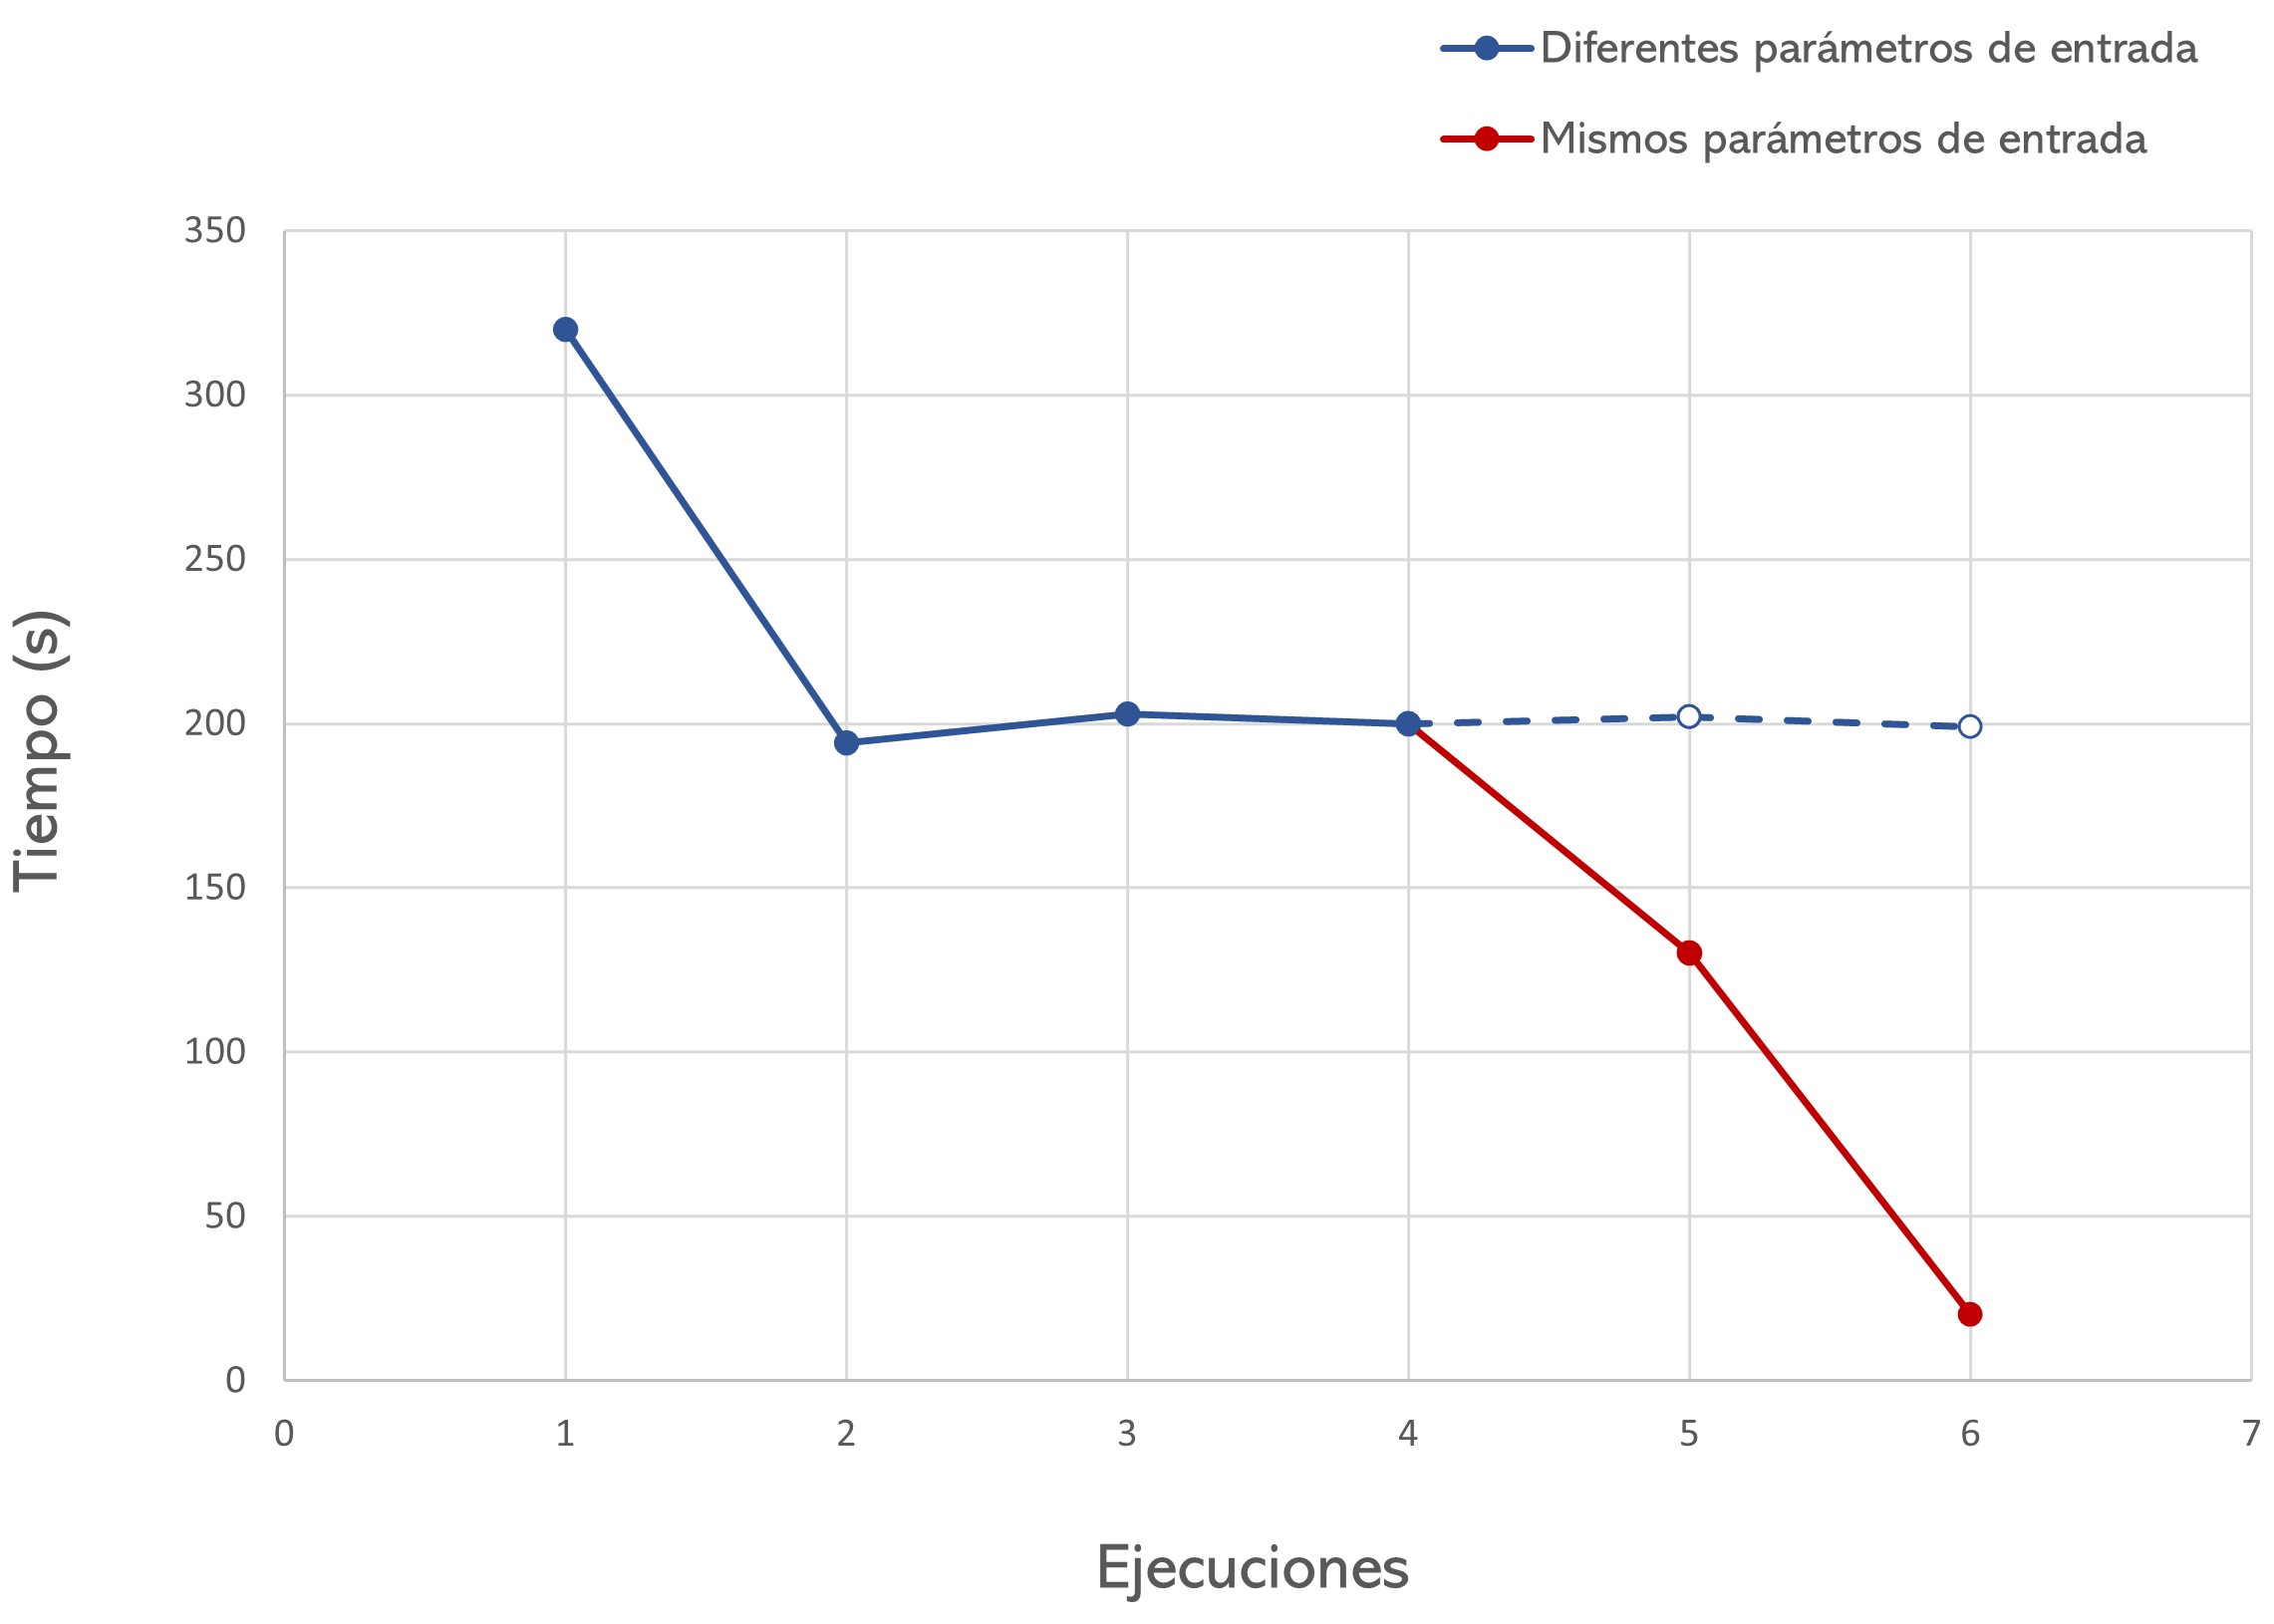
\includegraphics[width=13cm]{figuras/graph-times}}
  \caption{Tiempos de ejecución, con y sin cambios en el código de la aplicación entre ejecuciones.}
  \label{fig:times}
\end{figure}

Por lo tanto, se puede observar la buena gestión que Dagger hace de la caché. Es capaz de reducir un tercio el tiempo de ejecución de la misma función, con cambios en el código entro ejecuciones. En el caso de realizar pruebas sin hacer cambios en los parámetros de entrada, el tiempo de ejecución se reduce un 94\%. Este último valor de 20 segundos no es realista para el caso de uso de estos módulos, donde la entrada de las funciones (el código fuente) debería cambiar constantemente. Sin embargo, puede ser muy útil conocer esta capacidad de Dagger para aplicarlo en otras situaciones.

\section{Prueba 2}

La finalidad de esta prueba es comparar cómo se gestionan acciones básicas en el desarrollo de \textit{software}, como son la construcción de la aplicación y la ejecución de tests, tanto utilizando el módulo de Dagger como sin usarlo. Por lo tanto, se busca un resultado cualitativo, en el que lo importante reside en la facilidad del desarrollador para implementar y mantener lo necesario para llevar a cabo dichas acciones.

El módulo de Dagger de CI es el encargado de realizar las acciones comentadas. Se proporciona una función de construcción y de ejecución de tests para cada uno de los paquetes. El ciclo de construcción y testeo de la aplicación está creado íntegramente utilizando un único lenguaje de programación, lo cual ofrece simplicidad tanto a la hora de la implementación como del mantenimiento. Se puede utilizar lógica de programación para adaptar el \textit{pipeline} a distintos escenarios. El desarrollador también puede reutilizar código de manera muy sencilla, mediante la creación de funciones, a las cuales se las puede llamar desde cualquier sitio. El código está organizado y se previene la duplicación de lógica de programación.

La ejecución del módulo se puede hacer de manera local gracias a que Dagger lanza sus funciones sobre un \textit{runtime} de OCI, como Docker. Dagger también facilita la reproducibilidad gracias a que construye grafos para definir dependencias entre funciones, donde cada nodo del grafo define su entrada y su salida. Además, lo anterior también permite gestionar de mejor manera la caché, haciendo que las ejecuciones sean más rápidas, como ya se ha visto en la primera prueba de este capítulo.

En el caso de que no se use Dagger, el desarrollador tendría que optar por métodos convencionales. Comenzaría por crear un \texttt{Dockerfile} que permitiera realizar la construcción de los paquetes de la aplicación. Para realizar los tests del \textit{frontend}, haría falta otro \texttt{Dockerfile} específico para utilizar Cypress. Estos tests implicarían también implementar un archivo de Docker Compose, el cual permite levantar todos los servicios al mismo tiempo con posibilidad de comunicación entre ellos, necesario para realizar los tests \textit{end-to-end} del \textit{frontend}. 

Además, extender la lógica de programación implicaría crear \textit{scripts}, los cuales habría que acomodar a un nuevo entorno de desarrollo en el caso de que este cambie en algún momento. Esto añade más carga al desarrollador, que tiene que mantener dichos \textit{scripts} a lo largo de los diferentes entornos en los que se quieran ejecutar. Crear diferentes \textit{scripts} hace la reutilización de código más complicada, y puede llevar a la duplicación de lógica de programación. Finalmente, también se encuentra el problema de la reproducibilidad, siendo esto más complicado de conseguir debido a las pequeñas diferencias que pueda haber en la configuración del entorno de desarrollo de cada programador.

Sin embargo, la realidad es que las tecnologías y herramientas que se utilizan de manera convencional son más conocidas que Dagger. Por lo tanto, inicialmente puede ser lógico encaminarse por el uso de estas tecnologías, ya que permite iniciar la implementación de este tipo de ciclos más rápidamente. Además, aunque la API de Dagger es intuitiva si ya conoces las otras herramientas convencionales, su amplitud introduce una pequeña curva de aprendizaje. Pero, como se ha comentado, el mantenimiento a la larga es más sencillo con Dagger, debido a que todo se encuentra en un mismo lugar e implementado con un mismo lenguaje de programación, como Go, Python o Typescript (entre otros). Y, lo más importante, Dagger tiene una gran capacidad de portabilidad gracias a que ejecuta todas las funciones en entornos aislados, como los contenedores de Docker. Esto es una ventaja frente a los \textit{scripts}, que es necesario mantener en diferentes entornos en el caso de que no se utilice Dagger.

En la Tabla \ref{table:differences} se proporciona una tabla a modo de resumen, con las diferencias que se encuentran entre las dos opciones de implementación que se han comentado.

\begin{table}[htbp]
  \begin{tabularx}{\textwidth}{|>{\hsize=.75\hsize}X|X|>{\hsize=1.25\hsize}X|}
    \hline
    \textit{Aspecto} & \textit{Con Dagger} & \textit{Con métodos convencionales} \\ \hline
    Configuración inicial & Requiere un mayor esfuerzo para aprender su API & Más rápido de implementar al utilizar herramientas conocidas \\ \hline
    Mantenimiento & Centralizado en un solo lenguaje; facilita la reutilización y evita duplicación & Requiere mantener múltiples archivos, lo cual es propenso a inconsistencias \\ \hline
    Reproducibilidad & Alta, gracias a la ejecución en entornos aislados & Menor, debido a las posibles diferencias entre entornos locales de desarrollo \\ \hline
    Flexibilidad & Alta, permitiendo aplicar lógica de programación a todo el \textit{pipeline} & Limitada por la necesidad de creación y adaptación de diferentes \textit{scripts} \\ \hline
    Caché & Optimizada de forma automática & Manual, más dificil de mantener y optimizar \\ \hline
    Portabilidad & Elevada, todo se ejecuta en contenedores & Menor, requiere adaptar \textit{scripts} o configuraciones según el entorno \\ \hline
    Escalabilidad & Adecuado para cualquier proyecto, destacando en aquellos más grandes & Difícil de escalar conforme crece la lógica \\ \hline
    Curva de aprendizaje & Moderada, API extensa pero intuitiva si se tiene experiencia previa con contenedores & Baja, herramientas ampliamente conocidas \\ \hline
    Madurez del ecosistema & En crecimiento activo & Herramientas maduras con amplia documentación y soporte \\ \hline
  \end{tabularx}
  \caption{Diferencias entre Dagger y métodos convencionales.}
  \label{table:differences}
\end{table}
